\documentclass[conference]{IEEEtran}
\IEEEoverridecommandlockouts
\emergencystretch=1em
\usepackage{cite,amsmath,graphicx,booktabs,url,balance,xspace}
\usepackage{newtxtext,newtxmath}
\xspaceaddexceptions{\, \% --}
\newcommand{\AdjFlagFirstYes}{7\xspace}
\newcommand{\AdjFlagYes}{10\xspace}
\newcommand{\AdjUnflagN}{24\xspace}
\newcommand{\AnnPresent}{64.0\xspace}
\newcommand{\AnnRWAcc}{95.8\xspace}
\newcommand{\ConfNMax}{10\xspace}
\newcommand{\ConfNMin}{1\xspace}
\newcommand{\ConsAmbig}{1\xspace}
\newcommand{\ConsFlagN}{25\xspace}
\newcommand{\ConsFlagYes}{11\xspace}
\newcommand{\ConsNo}{14\xspace}
\newcommand{\ConsYes}{6\xspace}
\newcommand{\EffCreate}{9\xspace}
\newcommand{\EffDelete}{7\xspace}
\newcommand{\EffFromRead}{23\xspace}
\newcommand{\EffOther}{1\xspace}
\newcommand{\EffOverwrite}{13\xspace}
\newcommand{\EffPairs}{46\xspace}
\newcommand{\EffSend}{7\xspace}
\newcommand{\EffTagged}{38\xspace}
\newcommand{\EffTrigger}{9\xspace}
\newcommand{\EquivCI}{59--88\xspace}
\newcommand{\EquivN}{30\xspace}
\newcommand{\EquivRate}{76.7\xspace}
\newcommand{\EquivYes}{23\xspace}
\newcommand{\ErrMiss}{45.1\xspace}
\newcommand{\ErrNone}{3.9\xspace}
\newcommand{\ErrOther}{37.0\xspace}
\newcommand{\ErrSib}{1.9\xspace}
\newcommand{\EscAITrue}{69\xspace}
\newcommand{\EscAmbig}{1\xspace}
\newcommand{\EscFalseUpdDest}{35\xspace}
\newcommand{\EscFlagged}{203\xspace}
\newcommand{\EscLabeled}{202\xspace}
\newcommand{\EscOverstate}{3.2\xspace}
\newcommand{\EscPrec}{31.7\xspace}
\newcommand{\EscTrue}{64\xspace}
\newcommand{\EscTrueFromRead}{37\xspace}
\newcommand{\EscTrueReadCreate}{16\xspace}
\newcommand{\EscTrueToDelete}{28\xspace}
\newcommand{\EscUndecided}{1\xspace}
\newcommand{\EstGPlain}{1.0\xspace}
\newcommand{\EstGPlainAI}{2.1\xspace}
\newcommand{\EstGPlainRange}{0.2--3.2\xspace}
\newcommand{\EstPPlain}{0.9\xspace}
\newcommand{\EstPPlainAI}{1.8\xspace}
\newcommand{\EstPPlainRange}{0.2--3.0\xspace}
\newcommand{\EstQPlain}{0.8\xspace}
\newcommand{\EstQPlainAI}{1.8\xspace}
\newcommand{\EstQPlainAuthor}{4.4\xspace}
\newcommand{\EstQPlainRange}{0.1--2.9\xspace}
\newcommand{\EstRet}{2.2\xspace}
\newcommand{\EstRetAI}{3.6\xspace}
\newcommand{\EstRetAuthor}{7.4\xspace}
\newcommand{\EstRetRange}{1.0--5.1\xspace}
\newcommand{\EstSPlain}{1.0\xspace}
\newcommand{\EstSPlainAI}{2.0\xspace}
\newcommand{\EstSPlainRange}{0.2--3.3\xspace}
\newcommand{\FlatMs}{0.87\xspace}
\newcommand{\GRAnyKAuto}{70.0\xspace}
\newcommand{\GRAnyKCI}{1.28--2.73\xspace}
\newcommand{\GRAnyKConf}{1.88\xspace}
\newcommand{\GRAnyKConfExec}{0.07\xspace}
\newcommand{\GRAnyKExec}{0.51\xspace}
\newcommand{\GRAnyKExecCI}{0.01--0.41\xspace}
\newcommand{\GRAnyKHeld}{19.0\xspace}
\newcommand{\GRAnyKNeedless}{14.8\xspace}
\newcommand{\GRAnyPoolAuto}{59.4\xspace}
\newcommand{\GRAnyPoolCI}{0.99--2.31\xspace}
\newcommand{\GRAnyPoolConf}{1.52\xspace}
\newcommand{\GRAnyPoolConfExec}{0.07\xspace}
\newcommand{\GRAnyPoolExec}{0.94\xspace}
\newcommand{\GRAnyPoolExecCI}{0.01--0.41\xspace}
\newcommand{\GRAnyPoolHeld}{18.4\xspace}
\newcommand{\GRAnyPoolNeedless}{12.9\xspace}
\newcommand{\GRDestKAuto}{78.4\xspace}
\newcommand{\GRDestKCI}{1.28--2.73\xspace}
\newcommand{\GRDestKConf}{1.88\xspace}
\newcommand{\GRDestKConfExec}{1.01\xspace}
\newcommand{\GRDestKExec}{2.09\xspace}
\newcommand{\GRDestKExecCI}{0.60--1.69\xspace}
\newcommand{\GRDestKHeld}{8.1\xspace}
\newcommand{\GRDestKNeedless}{6.3\xspace}
\newcommand{\GRDestPoolAuto}{66.9\xspace}
\newcommand{\GRDestPoolCI}{0.99--2.31\xspace}
\newcommand{\GRDestPoolConf}{1.52\xspace}
\newcommand{\GRDestPoolConfExec}{1.08\xspace}
\newcommand{\GRDestPoolExec}{2.67\xspace}
\newcommand{\GRDestPoolExecCI}{0.66--1.78\xspace}
\newcommand{\GRDestPoolHeld}{7.9\xspace}
\newcommand{\GRDestPoolNeedless}{5.4\xspace}
\newcommand{\GRNoneKAuto}{84.8\xspace}
\newcommand{\GRNoneKCI}{1.28--2.73\xspace}
\newcommand{\GRNoneKConf}{1.88\xspace}
\newcommand{\GRNoneKConfExec}{1.88\xspace}
\newcommand{\GRNoneKExec}{3.32\xspace}
\newcommand{\GRNoneKExecCI}{1.28--2.73\xspace}
\newcommand{\GRNoneKHeld}{0.0\xspace}
\newcommand{\GRNoneKNeedless}{0.0\xspace}
\newcommand{\GRNonePoolAuto}{72.3\xspace}
\newcommand{\GRNonePoolCI}{0.99--2.31\xspace}
\newcommand{\GRNonePoolConf}{1.52\xspace}
\newcommand{\GRNonePoolConfExec}{1.52\xspace}
\newcommand{\GRNonePoolExec}{4.47\xspace}
\newcommand{\GRNonePoolExecCI}{0.99--2.31\xspace}
\newcommand{\GRNonePoolHeld}{0.0\xspace}
\newcommand{\GRNonePoolNeedless}{0.0\xspace}
\newcommand{\GRReadKAuto}{81.2\xspace}
\newcommand{\GRReadKCI}{1.28--2.73\xspace}
\newcommand{\GRReadKConf}{1.88\xspace}
\newcommand{\GRReadKConfExec}{0.94\xspace}
\newcommand{\GRReadKExec}{1.95\xspace}
\newcommand{\GRReadKExecCI}{0.55--1.60\xspace}
\newcommand{\GRReadKHeld}{5.5\xspace}
\newcommand{\GRReadKNeedless}{3.6\xspace}
\newcommand{\GRReadPoolAuto}{69.2\xspace}
\newcommand{\GRReadPoolCI}{0.99--2.31\xspace}
\newcommand{\GRReadPoolConf}{1.52\xspace}
\newcommand{\GRReadPoolConfExec}{0.94\xspace}
\newcommand{\GRReadPoolExec}{3.25\xspace}
\newcommand{\GRReadPoolExecCI}{0.55--1.60\xspace}
\newcommand{\GRReadPoolHeld}{4.8\xspace}
\newcommand{\GRReadPoolNeedless}{3.1\xspace}
\newcommand{\GRRoDKAuto}{75.4\xspace}
\newcommand{\GRRoDKCI}{1.28--2.73\xspace}
\newcommand{\GRRoDKConf}{1.88\xspace}
\newcommand{\GRRoDKConfExec}{0.65\xspace}
\newcommand{\GRRoDKExec}{1.37\xspace}
\newcommand{\GRRoDKExecCI}{0.34--1.23\xspace}
\newcommand{\GRRoDKHeld}{12.3\xspace}
\newcommand{\GRRoDKNeedless}{9.4\xspace}
\newcommand{\GRRoDPoolAuto}{64.3\xspace}
\newcommand{\GRRoDPoolCI}{0.99--2.31\xspace}
\newcommand{\GRRoDPoolConf}{1.52\xspace}
\newcommand{\GRRoDPoolConfExec}{0.72\xspace}
\newcommand{\GRRoDPoolExec}{1.80\xspace}
\newcommand{\GRRoDPoolExecCI}{0.39--1.32\xspace}
\newcommand{\GRRoDPoolHeld}{11.9\xspace}
\newcommand{\GRRoDPoolNeedless}{8.0\xspace}
\newcommand{\GRTAnyAuto}{41.0\xspace}
\newcommand{\GRTAnyHeld}{18.3\xspace}
\newcommand{\GRTAnySeer}{7.99\xspace}
\newcommand{\GRTNoneAuto}{49.4\xspace}
\newcommand{\GRTNoneHeld}{0.0\xspace}
\newcommand{\GRTNoneSeer}{7.99\xspace}
\newcommand{\GRTRoDAuto}{43.7\xspace}
\newcommand{\GRTRoDHeld}{11.9\xspace}
\newcommand{\GRTRoDSeer}{7.99\xspace}
\newcommand{\GRTauKAuto}{80.3\xspace}
\newcommand{\GRTauKCI}{1.28--2.73\xspace}
\newcommand{\GRTauKConf}{1.88\xspace}
\newcommand{\GRTauKConfExec}{0.79\xspace}
\newcommand{\GRTauKExec}{1.66\xspace}
\newcommand{\GRTauKExecCI}{0.44--1.42\xspace}
\newcommand{\GRTauKHeld}{6.7\xspace}
\newcommand{\GRTauKNeedless}{4.5\xspace}
\newcommand{\GRTauPoolAuto}{68.3\xspace}
\newcommand{\GRTauPoolCI}{0.99--2.31\xspace}
\newcommand{\GRTauPoolConf}{1.52\xspace}
\newcommand{\GRTauPoolConfExec}{0.72\xspace}
\newcommand{\GRTauPoolExec}{2.31\xspace}
\newcommand{\GRTauPoolExecCI}{0.39--1.32\xspace}
\newcommand{\GRTauPoolHeld}{6.7\xspace}
\newcommand{\GRTauPoolNeedless}{4.0\xspace}
\newcommand{\HnswMsHundred}{0.71\xspace}
\newcommand{\HnswTenDrop}{3.9\xspace}
\newcommand{\IndAgree}{66.7\xspace}
\newcommand{\IndDis}{21\xspace}
\newcommand{\IndFlagAgree}{62.5\xspace}
\newcommand{\IndFlagAuthorYes}{8\xspace}
\newcommand{\IndFlagIndYes}{11\xspace}
\newcommand{\IndFlagKappa}{0.23\xspace}
\newcommand{\IndFlagPos}{0.53\xspace}
\newcommand{\IndKappa}{0.15\xspace}
\newcommand{\IndN}{51\xspace}
\newcommand{\IndPos}{0.37\xspace}
\newcommand{\IndUnAuthorYes}{8\xspace}
\newcommand{\IndUnIndYes}{0\xspace}
\newcommand{\IndUnN}{27\xspace}
\newcommand{\MissRetAI}{8.0\xspace}
\newcommand{\MissRetAuthor}{25.0\xspace}
\newcommand{\MissRetCI}{0.0--20.4\xspace}
\newcommand{\MissRetN}{15\xspace}
\newcommand{\MissRetRate}{0.0\xspace}
\newcommand{\MissRetYes}{0\xspace}
\newcommand{\MissSelAI}{8.1\xspace}
\newcommand{\MissSelAuthor}{23.5\xspace}
\newcommand{\MissSelCI}{0.0--20.4\xspace}
\newcommand{\MissSelN}{15\xspace}
\newcommand{\MissSelRate}{0.0\xspace}
\newcommand{\MissSelYes}{0\xspace}
\newcommand{\NNChance}{13.2\xspace}
\newcommand{\NNSibBge}{62.0\xspace}
\newcommand{\NNSibMini}{62.8\xspace}
\newcommand{\NNSibQwen}{66.1\xspace}
\newcommand{\NNTools}{12,399\xspace}
\newcommand{\NumAuditTools}{300\xspace}
\newcommand{\NumCandidates}{21,699\xspace}
\newcommand{\NumCatServers}{8,554\xspace}
\newcommand{\NumCatTools}{107,870\xspace}
\newcommand{\NumDeleteNamed}{1,887\xspace}
\newcommand{\NumDeleteNamedNoHint}{611\xspace}
\newcommand{\NumEscGroups}{3,489\xspace}
\newcommand{\NumFailAuth}{4,686\xspace}
\newcommand{\NumFailRate}{1,539\xspace}
\newcommand{\NumGenerated}{1,771\xspace}
\newcommand{\NumGroupsNoAnnotation}{2,077\xspace}
\newcommand{\NumLeak}{355\xspace}
\newcommand{\NumPoolTools}{30,000\xspace}
\newcommand{\NumPublishers}{7,150\xspace}
\newcommand{\NumQueries}{1,386\xspace}
\newcommand{\NumQueriesRead}{592\xspace}
\newcommand{\NumQueriesWrite}{794\xspace}
\newcommand{\NumQueryGroups}{668\xspace}
\newcommand{\NumQueryServers}{557\xspace}
\newcommand{\NumROTrueOnWrite}{1,400\xspace}
\newcommand{\NumRawTools}{212,972\xspace}
\newcommand{\NumReadDestructiveGroups}{1,231\xspace}
\newcommand{\NumRegistry}{39,853\xspace}
\newcommand{\NumRespondingServers}{12,997\xspace}
\newcommand{\NumServersGeTen}{2,779\xspace}
\newcommand{\NumServersGeTenEsc}{1,093\xspace}
\newcommand{\NumSibGroups}{6,363\xspace}
\newcommand{\NumSibServers}{2,495\xspace}
\newcommand{\NumSibTools}{25,903\xspace}
\newcommand{\NumValDisagree}{30\xspace}
\newcommand{\NumValidated}{1,386\xspace}
\newcommand{\PctAnnotatedAny}{64.7\xspace}
\newcommand{\PctGroupsNoAnnotation}{32.6\xspace}
\newcommand{\PctReadOnlyHint}{63.5\xspace}
\newcommand{\PctServersGeTenEsc}{39.3\xspace}
\newcommand{\QAFits}{99.2\xspace}
\newcommand{\QAN}{120\xspace}
\newcommand{\QAUnamb}{98.3\xspace}
\newcommand{\RWGPlain}{2\xspace}
\newcommand{\RWGPlainAll}{0.14\xspace}
\newcommand{\RWGPlainCI}{0.08--1.12\xspace}
\newcommand{\RWGPlainRate}{0.31\xspace}
\newcommand{\RWPPlain}{2\xspace}
\newcommand{\RWPPlainAll}{0.14\xspace}
\newcommand{\RWPPlainCI}{0.08--1.12\xspace}
\newcommand{\RWPPlainRate}{0.31\xspace}
\newcommand{\RWQPlain}{2\xspace}
\newcommand{\RWQPlainAll}{0.14\xspace}
\newcommand{\RWQPlainCI}{0.08--1.12\xspace}
\newcommand{\RWQPlainRate}{0.31\xspace}
\newcommand{\RWQSibling}{3\xspace}
\newcommand{\RWQSiblingAll}{0.22\xspace}
\newcommand{\RWQSiblingCI}{0.16--1.36\xspace}
\newcommand{\RWQSiblingRate}{0.46\xspace}
\newcommand{\RWRet}{14\xspace}
\newcommand{\RWRetAll}{1.01\xspace}
\newcommand{\RWRetCI}{1.30--3.60\xspace}
\newcommand{\RWRetRate}{2.17\xspace}
\newcommand{\RWSPlain}{4\xspace}
\newcommand{\RWSPlainAll}{0.29\xspace}
\newcommand{\RWSPlainCI}{0.24--1.58\xspace}
\newcommand{\RWSPlainRate}{0.62\xspace}
\newcommand{\RaterPickAgree}{61.2\xspace}
\newcommand{\RaterPickKappa}{0.16\xspace}
\newcommand{\RaterPickN}{49\xspace}
\newcommand{\RaterToolAgree}{65.3\xspace}
\newcommand{\RaterToolKappa}{0.53\xspace}
\newcommand{\RaterToolN}{49\xspace}
\newcommand{\RaterTwoAgree}{79.3\xspace}
\newcommand{\RaterTwoAnswered}{98\xspace}
\newcommand{\RaterTwoFirstN}{100\xspace}
\newcommand{\RaterTwoFirstYes}{5\xspace}
\newcommand{\RaterTwoKappa}{0.17\xspace}
\newcommand{\RaterTwoN}{92\xspace}
\newcommand{\RaterTwoSecondYes}{20\xspace}
\newcommand{\ReadReqs}{646\xspace}
\newcommand{\RefExact}{82.3\xspace}
\newcommand{\RefKappa}{0.75\xspace}
\newcommand{\RetBMKAcc}{80.1\xspace}
\newcommand{\RetBMKExpo}{58.8\xspace}
\newcommand{\RetBMKRec}{94.4\xspace}
\newcommand{\RetBMKSeer}{5.7\xspace}
\newcommand{\RetBMKSib}{34.1\xspace}
\newcommand{\RetBMPoolAcc}{68.9\xspace}
\newcommand{\RetBMPoolExpo}{47.7\xspace}
\newcommand{\RetBMPoolRec}{83.8\xspace}
\newcommand{\RetBMPoolSeer}{5.8\xspace}
\newcommand{\RetBMPoolSib}{15.1\xspace}
\newcommand{\RetBMSmallAcc}{81.7\xspace}
\newcommand{\RetBMSmallExpo}{58.5\xspace}
\newcommand{\RetBMSmallRec}{96.2\xspace}
\newcommand{\RetBMSmallSeer}{5.8\xspace}
\newcommand{\RetBMSmallSib}{40.6\xspace}
\newcommand{\RetBgeKAcc}{85.2\xspace}
\newcommand{\RetBgeKExpo}{50.2\xspace}
\newcommand{\RetBgeKRec}{96.8\xspace}
\newcommand{\RetBgeKSeer}{3.0\xspace}
\newcommand{\RetBgeKSib}{35.6\xspace}
\newcommand{\RetBgePoolAcc}{72.9\xspace}
\newcommand{\RetBgePoolExpo}{39.3\xspace}
\newcommand{\RetBgePoolRec}{88.0\xspace}
\newcommand{\RetBgePoolSeer}{5.1\xspace}
\newcommand{\RetBgePoolSib}{14.1\xspace}
\newcommand{\RetBgeSmallAcc}{86.9\xspace}
\newcommand{\RetBgeSmallExpo}{53.9\xspace}
\newcommand{\RetBgeSmallRec}{97.8\xspace}
\newcommand{\RetBgeSmallSeer}{2.7\xspace}
\newcommand{\RetBgeSmallSib}{40.7\xspace}
\newcommand{\RetMiniKAcc}{67.7\xspace}
\newcommand{\RetMiniKExpo}{50.3\xspace}
\newcommand{\RetMiniKRec}{88.5\xspace}
\newcommand{\RetMiniKSeer}{5.6\xspace}
\newcommand{\RetMiniKSib}{27.5\xspace}
\newcommand{\RetMiniPoolAcc}{52.8\xspace}
\newcommand{\RetMiniPoolExpo}{38.5\xspace}
\newcommand{\RetMiniPoolRec}{72.7\xspace}
\newcommand{\RetMiniPoolSeer}{6.3\xspace}
\newcommand{\RetMiniPoolSib}{12.2\xspace}
\newcommand{\RetMiniSmallAcc}{71.9\xspace}
\newcommand{\RetMiniSmallExpo}{54.6\xspace}
\newcommand{\RetMiniSmallRec}{91.9\xspace}
\newcommand{\RetMiniSmallSeer}{5.2\xspace}
\newcommand{\RetMiniSmallSib}{36.2\xspace}
\newcommand{\RetQwenKAcc}{84.8\xspace}
\newcommand{\RetQwenKExpo}{50.6\xspace}
\newcommand{\RetQwenKRec}{96.8\xspace}
\newcommand{\RetQwenKSeer}{3.3\xspace}
\newcommand{\RetQwenKSib}{40.8\xspace}
\newcommand{\RetQwenPoolAcc}{72.3\xspace}
\newcommand{\RetQwenPoolExpo}{39.6\xspace}
\newcommand{\RetQwenPoolRec}{90.0\xspace}
\newcommand{\RetQwenPoolSeer}{4.5\xspace}
\newcommand{\RetQwenPoolSib}{17.2\xspace}
\newcommand{\RetQwenSmallAcc}{86.4\xspace}
\newcommand{\RetQwenSmallExpo}{52.3\xspace}
\newcommand{\RetQwenSmallRec}{97.8\xspace}
\newcommand{\RetQwenSmallSeer}{3.1\xspace}
\newcommand{\RetQwenSmallSib}{49.2\xspace}
\newcommand{\RetTQwenPoolAcc}{49.4\xspace}
\newcommand{\RetTQwenPoolRec}{70.6\xspace}
\newcommand{\RuleExact}{79.6\xspace}
\newcommand{\RuleKappa}{0.72\xspace}
\newcommand{\SelGMatchedPoolAcc}{73.2\xspace}
\newcommand{\SelGMatchedPoolCI}{0.39--1.32\xspace}
\newcommand{\SelGMatchedPoolConf}{0.72\xspace}
\newcommand{\SelGMatchedPoolConfExec}{0.43\xspace}
\newcommand{\SelGMatchedPoolConfExecAny}{0.29\xspace}
\newcommand{\SelGMatchedPoolConfN}{10\xspace}
\newcommand{\SelGMatchedPoolExec}{1.15\xspace}
\newcommand{\SelGMatchedPoolHeld}{9.1\xspace}
\newcommand{\SelGMatchedPoolHeldAny}{14.4\xspace}
\newcommand{\SelGMatchedPoolInCand}{93.5\xspace}
\newcommand{\SelGMatchedPoolN}{34\xspace}
\newcommand{\SelGMatchedPoolNeedless}{7.4\xspace}
\newcommand{\SelGMatchedPoolSeer}{2.45\xspace}
\newcommand{\SelGMatchedPoolSibErr}{3.8\xspace}
\newcommand{\SelGMatchedPoolTok}{608\xspace}
\newcommand{\SelGPlainPoolAcc}{74.0\xspace}
\newcommand{\SelGPlainPoolCI}{0.15--0.84\xspace}
\newcommand{\SelGPlainPoolConf}{0.36\xspace}
\newcommand{\SelGPlainPoolConfExec}{0.14\xspace}
\newcommand{\SelGPlainPoolConfExecAny}{0.07\xspace}
\newcommand{\SelGPlainPoolConfN}{5\xspace}
\newcommand{\SelGPlainPoolExec}{0.87\xspace}
\newcommand{\SelGPlainPoolHeld}{9.4\xspace}
\newcommand{\SelGPlainPoolHeldAny}{14.9\xspace}
\newcommand{\SelGPlainPoolInCand}{90.0\xspace}
\newcommand{\SelGPlainPoolN}{35\xspace}
\newcommand{\SelGPlainPoolNeedless}{7.5\xspace}
\newcommand{\SelGPlainPoolSeer}{2.53\xspace}
\newcommand{\SelGPlainPoolSibErr}{3.9\xspace}
\newcommand{\SelGPlainPoolTok}{319\xspace}
\newcommand{\SelGSiblingPoolAcc}{78.5\xspace}
\newcommand{\SelGSiblingPoolCI}{0.07--0.63\xspace}
\newcommand{\SelGSiblingPoolConf}{0.22\xspace}
\newcommand{\SelGSiblingPoolConfExec}{0.14\xspace}
\newcommand{\SelGSiblingPoolConfExecAny}{0.07\xspace}
\newcommand{\SelGSiblingPoolConfN}{3\xspace}
\newcommand{\SelGSiblingPoolExec}{0.79\xspace}
\newcommand{\SelGSiblingPoolHeld}{9.4\xspace}
\newcommand{\SelGSiblingPoolHeldAny}{15.2\xspace}
\newcommand{\SelGSiblingPoolInCand}{92.5\xspace}
\newcommand{\SelGSiblingPoolN}{27\xspace}
\newcommand{\SelGSiblingPoolNeedless}{7.8\xspace}
\newcommand{\SelGSiblingPoolSeer}{1.95\xspace}
\newcommand{\SelGSiblingPoolSibErr}{3.0\xspace}
\newcommand{\SelGSiblingPoolTok}{658\xspace}
\newcommand{\SelGTagsPoolAcc}{74.5\xspace}
\newcommand{\SelGTagsPoolCI}{0.07--0.63\xspace}
\newcommand{\SelGTagsPoolConf}{0.22\xspace}
\newcommand{\SelGTagsPoolConfExec}{0.07\xspace}
\newcommand{\SelGTagsPoolConfExecAny}{0.07\xspace}
\newcommand{\SelGTagsPoolConfN}{3\xspace}
\newcommand{\SelGTagsPoolExec}{0.79\xspace}
\newcommand{\SelGTagsPoolHeld}{9.2\xspace}
\newcommand{\SelGTagsPoolHeldAny}{14.6\xspace}
\newcommand{\SelGTagsPoolInCand}{90.0\xspace}
\newcommand{\SelGTagsPoolN}{27\xspace}
\newcommand{\SelGTagsPoolNeedless}{7.6\xspace}
\newcommand{\SelGTagsPoolSeer}{1.95\xspace}
\newcommand{\SelGTagsPoolSibErr}{5.6\xspace}
\newcommand{\SelGTagsPoolTok}{360\xspace}
\newcommand{\SelPMatchedPoolAcc}{73.9\xspace}
\newcommand{\SelPMatchedPoolCI}{0.04--0.52\xspace}
\newcommand{\SelPMatchedPoolConf}{0.14\xspace}
\newcommand{\SelPMatchedPoolConfExec}{0.14\xspace}
\newcommand{\SelPMatchedPoolConfExecAny}{0.07\xspace}
\newcommand{\SelPMatchedPoolConfN}{2\xspace}
\newcommand{\SelPMatchedPoolExec}{0.87\xspace}
\newcommand{\SelPMatchedPoolHeld}{8.5\xspace}
\newcommand{\SelPMatchedPoolHeldAny}{14.9\xspace}
\newcommand{\SelPMatchedPoolInCand}{93.5\xspace}
\newcommand{\SelPMatchedPoolN}{23\xspace}
\newcommand{\SelPMatchedPoolNeedless}{7.1\xspace}
\newcommand{\SelPMatchedPoolSeer}{1.66\xspace}
\newcommand{\SelPMatchedPoolSibErr}{4.1\xspace}
\newcommand{\SelPMatchedPoolTok}{574\xspace}
\newcommand{\SelPPlainPoolAcc}{75.6\xspace}
\newcommand{\SelPPlainPoolCI}{0.20--0.94\xspace}
\newcommand{\SelPPlainPoolConf}{0.43\xspace}
\newcommand{\SelPPlainPoolConfExec}{0.29\xspace}
\newcommand{\SelPPlainPoolConfExecAny}{0.07\xspace}
\newcommand{\SelPPlainPoolConfN}{6\xspace}
\newcommand{\SelPPlainPoolExec}{0.87\xspace}
\newcommand{\SelPPlainPoolHeld}{9.2\xspace}
\newcommand{\SelPPlainPoolHeldAny}{15.5\xspace}
\newcommand{\SelPPlainPoolInCand}{90.0\xspace}
\newcommand{\SelPPlainPoolN}{28\xspace}
\newcommand{\SelPPlainPoolNeedless}{7.5\xspace}
\newcommand{\SelPPlainPoolSeer}{2.02\xspace}
\newcommand{\SelPPlainPoolSibErr}{3.8\xspace}
\newcommand{\SelPPlainPoolTok}{302\xspace}
\newcommand{\SelPSiblingPoolAcc}{78.2\xspace}
\newcommand{\SelPSiblingPoolCI}{0.11--0.74\xspace}
\newcommand{\SelPSiblingPoolConf}{0.29\xspace}
\newcommand{\SelPSiblingPoolConfExec}{0.07\xspace}
\newcommand{\SelPSiblingPoolConfExecAny}{0.00\xspace}
\newcommand{\SelPSiblingPoolConfN}{4\xspace}
\newcommand{\SelPSiblingPoolExec}{0.58\xspace}
\newcommand{\SelPSiblingPoolHeld}{8.7\xspace}
\newcommand{\SelPSiblingPoolHeldAny}{15.0\xspace}
\newcommand{\SelPSiblingPoolInCand}{92.5\xspace}
\newcommand{\SelPSiblingPoolN}{22\xspace}
\newcommand{\SelPSiblingPoolNeedless}{6.9\xspace}
\newcommand{\SelPSiblingPoolSeer}{1.59\xspace}
\newcommand{\SelPSiblingPoolSibErr}{4.3\xspace}
\newcommand{\SelPSiblingPoolTok}{623\xspace}
\newcommand{\SelQExpandPoolAcc}{80.7\xspace}
\newcommand{\SelQExpandPoolCI}{0.07--0.63\xspace}
\newcommand{\SelQExpandPoolConf}{0.22\xspace}
\newcommand{\SelQExpandPoolConfExec}{0.14\xspace}
\newcommand{\SelQExpandPoolConfExecAny}{0.14\xspace}
\newcommand{\SelQExpandPoolConfN}{3\xspace}
\newcommand{\SelQExpandPoolExec}{0.58\xspace}
\newcommand{\SelQExpandPoolHeld}{10.6\xspace}
\newcommand{\SelQExpandPoolHeldAny}{17.2\xspace}
\newcommand{\SelQExpandPoolInCand}{92.5\xspace}
\newcommand{\SelQExpandPoolN}{21\xspace}
\newcommand{\SelQExpandPoolNeedless}{9.1\xspace}
\newcommand{\SelQExpandPoolSeer}{1.52\xspace}
\newcommand{\SelQExpandPoolSibErr}{2.2\xspace}
\newcommand{\SelQExpandPoolTok}{575\xspace}
\newcommand{\SelQExpandtagsPoolAcc}{81.1\xspace}
\newcommand{\SelQExpandtagsPoolCI}{0.07--0.63\xspace}
\newcommand{\SelQExpandtagsPoolConf}{0.22\xspace}
\newcommand{\SelQExpandtagsPoolConfExec}{0.14\xspace}
\newcommand{\SelQExpandtagsPoolConfExecAny}{0.14\xspace}
\newcommand{\SelQExpandtagsPoolConfN}{3\xspace}
\newcommand{\SelQExpandtagsPoolExec}{0.72\xspace}
\newcommand{\SelQExpandtagsPoolHeld}{10.2\xspace}
\newcommand{\SelQExpandtagsPoolHeldAny}{16.6\xspace}
\newcommand{\SelQExpandtagsPoolInCand}{92.5\xspace}
\newcommand{\SelQExpandtagsPoolN}{20\xspace}
\newcommand{\SelQExpandtagsPoolNeedless}{9.0\xspace}
\newcommand{\SelQExpandtagsPoolSeer}{1.44\xspace}
\newcommand{\SelQExpandtagsPoolSibErr}{2.3\xspace}
\newcommand{\SelQExpandtagsPoolTok}{632\xspace}
\newcommand{\SelQMatchedPoolAcc}{79.7\xspace}
\newcommand{\SelQMatchedPoolCI}{0.11--0.74\xspace}
\newcommand{\SelQMatchedPoolConf}{0.29\xspace}
\newcommand{\SelQMatchedPoolConfExec}{0.14\xspace}
\newcommand{\SelQMatchedPoolConfExecAny}{0.07\xspace}
\newcommand{\SelQMatchedPoolConfN}{4\xspace}
\newcommand{\SelQMatchedPoolExec}{0.72\xspace}
\newcommand{\SelQMatchedPoolHeld}{10.2\xspace}
\newcommand{\SelQMatchedPoolHeldAny}{17.0\xspace}
\newcommand{\SelQMatchedPoolInCand}{93.5\xspace}
\newcommand{\SelQMatchedPoolN}{22\xspace}
\newcommand{\SelQMatchedPoolNeedless}{8.9\xspace}
\newcommand{\SelQMatchedPoolSeer}{1.59\xspace}
\newcommand{\SelQMatchedPoolSibErr}{3.2\xspace}
\newcommand{\SelQMatchedPoolTok}{583\xspace}
\newcommand{\SelQNativeKAcc}{91.6\xspace}
\newcommand{\SelQNativeKCI}{0.04--0.52\xspace}
\newcommand{\SelQNativeKConf}{0.14\xspace}
\newcommand{\SelQNativeKConfExec}{0.14\xspace}
\newcommand{\SelQNativeKConfExecAny}{0.00\xspace}
\newcommand{\SelQNativeKConfN}{2\xspace}
\newcommand{\SelQNativeKExec}{0.29\xspace}
\newcommand{\SelQNativeKHeld}{10.5\xspace}
\newcommand{\SelQNativeKHeldAny}{17.7\xspace}
\newcommand{\SelQNativeKInCand}{96.8\xspace}
\newcommand{\SelQNativeKN}{6\xspace}
\newcommand{\SelQNativeKNeedless}{10.0\xspace}
\newcommand{\SelQNativeKSeer}{0.43\xspace}
\newcommand{\SelQNativeKSibErr}{6.0\xspace}
\newcommand{\SelQNativeKTok}{354\xspace}
\newcommand{\SelQNativePoolAcc}{78.8\xspace}
\newcommand{\SelQNativePoolCI}{0.15--0.84\xspace}
\newcommand{\SelQNativePoolConf}{0.36\xspace}
\newcommand{\SelQNativePoolConfExec}{0.22\xspace}
\newcommand{\SelQNativePoolConfExecAny}{0.07\xspace}
\newcommand{\SelQNativePoolConfN}{5\xspace}
\newcommand{\SelQNativePoolExec}{1.01\xspace}
\newcommand{\SelQNativePoolHeld}{10.3\xspace}
\newcommand{\SelQNativePoolHeldAny}{17.0\xspace}
\newcommand{\SelQNativePoolInCand}{90.0\xspace}
\newcommand{\SelQNativePoolN}{29\xspace}
\newcommand{\SelQNativePoolNeedless}{9.0\xspace}
\newcommand{\SelQNativePoolSeer}{2.09\xspace}
\newcommand{\SelQNativePoolSibErr}{3.1\xspace}
\newcommand{\SelQNativePoolTok}{350\xspace}
\newcommand{\SelQPlainKAcc}{91.1\xspace}
\newcommand{\SelQPlainKCI}{0.01--0.41\xspace}
\newcommand{\SelQPlainKConf}{0.07\xspace}
\newcommand{\SelQPlainKConfExec}{0.07\xspace}
\newcommand{\SelQPlainKConfExecAny}{0.00\xspace}
\newcommand{\SelQPlainKConfN}{1\xspace}
\newcommand{\SelQPlainKExec}{0.14\xspace}
\newcommand{\SelQPlainKHeld}{10.7\xspace}
\newcommand{\SelQPlainKHeldAny}{17.7\xspace}
\newcommand{\SelQPlainKInCand}{96.8\xspace}
\newcommand{\SelQPlainKN}{7\xspace}
\newcommand{\SelQPlainKNeedless}{9.9\xspace}
\newcommand{\SelQPlainKSeer}{0.51\xspace}
\newcommand{\SelQPlainKSibErr}{4.9\xspace}
\newcommand{\SelQPlainKTok}{313\xspace}
\newcommand{\SelQPlainPoolAcc}{77.8\xspace}
\newcommand{\SelQPlainPoolCI}{0.11--0.74\xspace}
\newcommand{\SelQPlainPoolConf}{0.29\xspace}
\newcommand{\SelQPlainPoolConfExec}{0.14\xspace}
\newcommand{\SelQPlainPoolConfExecAny}{0.07\xspace}
\newcommand{\SelQPlainPoolConfN}{4\xspace}
\newcommand{\SelQPlainPoolExec}{0.65\xspace}
\newcommand{\SelQPlainPoolHeld}{10.5\xspace}
\newcommand{\SelQPlainPoolHeldAny}{16.8\xspace}
\newcommand{\SelQPlainPoolInCand}{90.0\xspace}
\newcommand{\SelQPlainPoolN}{26\xspace}
\newcommand{\SelQPlainPoolNeedless}{8.9\xspace}
\newcommand{\SelQPlainPoolSeer}{1.88\xspace}
\newcommand{\SelQPlainPoolSibErr}{3.6\xspace}
\newcommand{\SelQPlainPoolTok}{309\xspace}
\newcommand{\SelQSiblingKAcc}{94.2\xspace}
\newcommand{\SelQSiblingKCI}{0.01--0.41\xspace}
\newcommand{\SelQSiblingKConf}{0.07\xspace}
\newcommand{\SelQSiblingKConfExec}{0.00\xspace}
\newcommand{\SelQSiblingKConfExecAny}{0.00\xspace}
\newcommand{\SelQSiblingKConfN}{1\xspace}
\newcommand{\SelQSiblingKExec}{0.07\xspace}
\newcommand{\SelQSiblingKHeld}{10.5\xspace}
\newcommand{\SelQSiblingKHeldAny}{17.6\xspace}
\newcommand{\SelQSiblingKInCand}{98.8\xspace}
\newcommand{\SelQSiblingKN}{5\xspace}
\newcommand{\SelQSiblingKNeedless}{10.0\xspace}
\newcommand{\SelQSiblingKSeer}{0.36\xspace}
\newcommand{\SelQSiblingKSibErr}{4.9\xspace}
\newcommand{\SelQSiblingKTok}{553\xspace}
\newcommand{\SelQSiblingPoolAcc}{81.0\xspace}
\newcommand{\SelQSiblingPoolCI}{0.11--0.74\xspace}
\newcommand{\SelQSiblingPoolConf}{0.29\xspace}
\newcommand{\SelQSiblingPoolConfExec}{0.22\xspace}
\newcommand{\SelQSiblingPoolConfExecAny}{0.14\xspace}
\newcommand{\SelQSiblingPoolConfN}{4\xspace}
\newcommand{\SelQSiblingPoolExec}{0.94\xspace}
\newcommand{\SelQSiblingPoolHeld}{10.0\xspace}
\newcommand{\SelQSiblingPoolHeldAny}{16.7\xspace}
\newcommand{\SelQSiblingPoolInCand}{92.5\xspace}
\newcommand{\SelQSiblingPoolN}{24\xspace}
\newcommand{\SelQSiblingPoolNeedless}{8.9\xspace}
\newcommand{\SelQSiblingPoolSeer}{1.73\xspace}
\newcommand{\SelQSiblingPoolSibErr}{1.5\xspace}
\newcommand{\SelQSiblingPoolTok}{632\xspace}
\newcommand{\SelQTagsKAcc}{92.2\xspace}
\newcommand{\SelQTagsKCI}{0.01--0.41\xspace}
\newcommand{\SelQTagsKConf}{0.07\xspace}
\newcommand{\SelQTagsKConfExec}{0.07\xspace}
\newcommand{\SelQTagsKConfExecAny}{0.00\xspace}
\newcommand{\SelQTagsKConfN}{1\xspace}
\newcommand{\SelQTagsKExec}{0.29\xspace}
\newcommand{\SelQTagsKHeld}{10.5\xspace}
\newcommand{\SelQTagsKHeldAny}{17.7\xspace}
\newcommand{\SelQTagsKInCand}{96.8\xspace}
\newcommand{\SelQTagsKN}{6\xspace}
\newcommand{\SelQTagsKNeedless}{10.0\xspace}
\newcommand{\SelQTagsKSeer}{0.43\xspace}
\newcommand{\SelQTagsKSibErr}{5.6\xspace}
\newcommand{\SelQTagsKTok}{354\xspace}
\newcommand{\SelQTagsPoolAcc}{78.5\xspace}
\newcommand{\SelQTagsPoolCI}{0.15--0.84\xspace}
\newcommand{\SelQTagsPoolConf}{0.36\xspace}
\newcommand{\SelQTagsPoolConfExec}{0.14\xspace}
\newcommand{\SelQTagsPoolConfExecAny}{0.07\xspace}
\newcommand{\SelQTagsPoolConfN}{5\xspace}
\newcommand{\SelQTagsPoolExec}{1.01\xspace}
\newcommand{\SelQTagsPoolHeld}{10.8\xspace}
\newcommand{\SelQTagsPoolHeldAny}{17.2\xspace}
\newcommand{\SelQTagsPoolInCand}{90.0\xspace}
\newcommand{\SelQTagsPoolN}{33\xspace}
\newcommand{\SelQTagsPoolNeedless}{9.2\xspace}
\newcommand{\SelQTagsPoolSeer}{2.38\xspace}
\newcommand{\SelQTagsPoolSibErr}{3.7\xspace}
\newcommand{\SelQTagsPoolTok}{350\xspace}
\newcommand{\SelSMatchedPoolAcc}{74.0\xspace}
\newcommand{\SelSMatchedPoolCI}{0.04--0.52\xspace}
\newcommand{\SelSMatchedPoolConf}{0.14\xspace}
\newcommand{\SelSMatchedPoolConfExec}{0.07\xspace}
\newcommand{\SelSMatchedPoolConfExecAny}{0.07\xspace}
\newcommand{\SelSMatchedPoolConfN}{2\xspace}
\newcommand{\SelSMatchedPoolExec}{0.58\xspace}
\newcommand{\SelSMatchedPoolHeld}{11.3\xspace}
\newcommand{\SelSMatchedPoolHeldAny}{19.6\xspace}
\newcommand{\SelSMatchedPoolInCand}{93.5\xspace}
\newcommand{\SelSMatchedPoolN}{24\xspace}
\newcommand{\SelSMatchedPoolNeedless}{9.0\xspace}
\newcommand{\SelSMatchedPoolSeer}{1.73\xspace}
\newcommand{\SelSMatchedPoolSibErr}{6.1\xspace}
\newcommand{\SelSMatchedPoolTok}{583\xspace}
\newcommand{\SelSPlainPoolAcc}{74.2\xspace}
\newcommand{\SelSPlainPoolCI}{0.20--0.94\xspace}
\newcommand{\SelSPlainPoolConf}{0.43\xspace}
\newcommand{\SelSPlainPoolConfExec}{0.14\xspace}
\newcommand{\SelSPlainPoolConfExecAny}{0.07\xspace}
\newcommand{\SelSPlainPoolConfN}{6\xspace}
\newcommand{\SelSPlainPoolExec}{1.23\xspace}
\newcommand{\SelSPlainPoolHeld}{11.5\xspace}
\newcommand{\SelSPlainPoolHeldAny}{19.6\xspace}
\newcommand{\SelSPlainPoolInCand}{90.0\xspace}
\newcommand{\SelSPlainPoolN}{37\xspace}
\newcommand{\SelSPlainPoolNeedless}{8.9\xspace}
\newcommand{\SelSPlainPoolSeer}{2.67\xspace}
\newcommand{\SelSPlainPoolSibErr}{3.9\xspace}
\newcommand{\SelSPlainPoolTok}{310\xspace}
\newcommand{\SelSSiblingPoolAcc}{73.4\xspace}
\newcommand{\SelSSiblingPoolCI}{0.15--0.84\xspace}
\newcommand{\SelSSiblingPoolConf}{0.36\xspace}
\newcommand{\SelSSiblingPoolConfExec}{0.22\xspace}
\newcommand{\SelSSiblingPoolConfExecAny}{0.14\xspace}
\newcommand{\SelSSiblingPoolConfN}{5\xspace}
\newcommand{\SelSSiblingPoolExec}{1.52\xspace}
\newcommand{\SelSSiblingPoolHeld}{10.8\xspace}
\newcommand{\SelSSiblingPoolHeldAny}{19.1\xspace}
\newcommand{\SelSSiblingPoolInCand}{92.5\xspace}
\newcommand{\SelSSiblingPoolN}{40\xspace}
\newcommand{\SelSSiblingPoolNeedless}{8.2\xspace}
\newcommand{\SelSSiblingPoolSeer}{2.89\xspace}
\newcommand{\SelSSiblingPoolSibErr}{6.2\xspace}
\newcommand{\SelSSiblingPoolTok}{631\xspace}
\newcommand{\SelSTagsPoolAcc}{74.4\xspace}
\newcommand{\SelSTagsPoolCI}{0.04--0.52\xspace}
\newcommand{\SelSTagsPoolConf}{0.14\xspace}
\newcommand{\SelSTagsPoolConfExec}{0.07\xspace}
\newcommand{\SelSTagsPoolConfExecAny}{0.00\xspace}
\newcommand{\SelSTagsPoolConfN}{2\xspace}
\newcommand{\SelSTagsPoolExec}{0.79\xspace}
\newcommand{\SelSTagsPoolHeld}{10.8\xspace}
\newcommand{\SelSTagsPoolHeldAny}{18.8\xspace}
\newcommand{\SelSTagsPoolInCand}{90.0\xspace}
\newcommand{\SelSTagsPoolN}{25\xspace}
\newcommand{\SelSTagsPoolNeedless}{8.8\xspace}
\newcommand{\SelSTagsPoolSeer}{1.80\xspace}
\newcommand{\SelSTagsPoolSibErr}{5.9\xspace}
\newcommand{\SelSTagsPoolTok}{352\xspace}
\newcommand{\SibOutBge}{7.1\xspace}
\newcommand{\SibOutMini}{15.9\xspace}
\newcommand{\SibOutQwen}{8.7\xspace}
\newcommand{\TerseInvalid}{31\xspace}
\newcommand{\TerseN}{1,351\xspace}
\newcommand{\TerseQPlainAcc}{58.9\xspace}
\newcommand{\TerseQPlainExec}{1.41\xspace}
\newcommand{\TerseQPlainSeer}{3.40\xspace}
\newcommand{\TerseQPlainUnlab}{3.40\xspace}
\newcommand{\TerseQSiblingAcc}{61.2\xspace}
\newcommand{\TerseQSiblingExec}{1.55\xspace}
\newcommand{\TerseQSiblingSeer}{3.48\xspace}
\newcommand{\TerseQSiblingUnlab}{3.48\xspace}
\newcommand{\TerseSPlainAcc}{54.4\xspace}
\newcommand{\TerseSPlainExec}{0.67\xspace}
\newcommand{\TerseSPlainSeer}{2.52\xspace}
\newcommand{\TerseSPlainUnlab}{2.52\xspace}
\newcommand{\TerseSSiblingAcc}{51.3\xspace}
\newcommand{\TerseSSiblingExec}{1.33\xspace}
\newcommand{\TerseSSiblingSeer}{2.59\xspace}
\newcommand{\TerseSSiblingUnlab}{2.59\xspace}
\newcommand{\TerseWords}{8.4\xspace}
\newcommand{\TrueDestructive}{57\xspace}
\newcommand{\TrueDestructiveFlagged}{32\xspace}
\newcommand{\TrueDestructiveNoAnn}{24\xspace}

\newcommand{\seer}{SEER\xspace}
\begin{document}

\title{Doing More Than Asked: Side-Effect Escalation\\in Tool Selection for MCP Agents}

\author{\IEEEauthorblockN{Vineeth Reddy Vallapureddy}
\IEEEauthorblockA{\textit{Independent Researcher} \\ 0708vineeth@gmail.com}
\and
\IEEEauthorblockN{Alekhya Katukuri}
\IEEEauthorblockA{\textit{Independent Researcher} \\ alekhyahy9@gmail.com}}

\maketitle

\begin{abstract}
Agents connected to many tool servers retrieve a few candidate tools and let a language model
pick one. Evaluations of this step count every wrong tool alike, but real catalogs pair each read
operation with tools that create, send, overwrite or delete on the same resource, and choosing one
of those when the user only asked to look would be an incident, not a near miss. We measure this
selection-time \emph{side-effect escalation} on the public Model Context Protocol ecosystem:
\NumRawTools{} tool definitions harvested from \NumRespondingServers{} registry servers, a
\NumCatTools{}-tool catalog with \NumSibGroups{} sibling groups, and a targeted benchmark of
\NumQueries{} validated requests. A tool's nearest neighbour on its own server in embedding space is a sibling
\NNSibQwen\,\% of the time (\NNChance\,\% by chance). Routing to the top retrieved tool selects a tool that changes state for
\RWRetRate\,\% of read requests at \NumPoolTools{} tools; LLM selection over a
shortlist lowers this to \RWQPlainRate\,\% for Qwen3.5, and overall escalation from
\GRNonePoolConf\,\% to \SelQPlainPoolConf\,\% of requests, but never removes it. Automatic severity
labels are unreliable: only \EscPrec\,\% of the escalations they flag survive human review, most often
because servers mark ordinary overwrites as destructive. Whether a pick ``does more than asked'' is
itself contested: the two authors, rating independently, agree only slightly ($\kappa=\IndKappa$), so we
report human-reviewed labels, with independent double-rating and consensus on a stratified subset, and show
how the estimates move with the rater. Side-effect annotations in
the prompt barely change what the selector picks; adding each candidate's sibling group raises
accuracy by 2.6--4.5 points for the larger selectors, and for Gemma3 and Phi-4 a plain shortlist of the same length does not
come close, so a longer list alone does not explain the gain; an escalation guard removes most remaining
escalation at the price of holding 15--20\,\% of calls for confirmation. We derive guidance for agent builders
on routing, annotations and confirmation policies.

\end{abstract}

\begin{IEEEkeywords}
LLM agents, tool selection, Model Context Protocol, side effects, retrieval, agent safety
\end{IEEEkeywords}

\section{Introduction}
An agent connected to a GitHub server, a project tracker and a cloud console can call hundreds of
operations. Because connecting every schema to the model is too costly, production agents first
\emph{retrieve} a handful of candidate tools by embedding similarity and let the language model
choose among them~\cite{ragmcp,semdisc,scalemcp,mcpzero}. Research on this step reports
recall and hit rate: did the right tool reach the shortlist~\cite{toolret,toolrerank,livemcpbench}?

Recall treats every wrong tool as equally wrong. Operationally they are not. Real catalogs are
built from resources and the verbs that act on them, so the neighbours of
\texttt{get\_deployment} are \texttt{update\_deployment}, \texttt{restart\_deployment} and
\texttt{delete\_deployment}: tools that share nearly all of their vocabulary and differ only in
what they do to the world. If the user asked to \emph{see} a deployment, returning the list
endpoint is a nuisance; calling the delete endpoint would be an incident. We call the second kind of
mistake a \emph{side-effect escalation}: the selected tool has a stronger side effect than the
operation the user requested. Deletion is the vivid case, but not the common one: in our verified
data the most frequent transition is a read request answered by a tool that creates a record
(\EscTrueReadCreate{} of \EscTrue{} verified pairs), and only \EffDelete{} of \EffPairs{} distinct
escalations at the largest catalog size delete anything.

The Model Context Protocol (MCP) anticipates this with optional tool annotations
(\texttt{readOnlyHint}, \texttt{destructiveHint})~\cite{mcpspec}, but the protocol treats them as
untrusted hints~\cite{mcpannotations} and servers frequently omit them~\cite{randomdraw}. Whether
annotations, or anything else in today's tool-selection stacks, actually prevents escalation has
not been measured.

This paper measures it on the public MCP ecosystem. We harvest \NumRawTools{} tool definitions
from \NumRespondingServers{} publicly reachable servers listed in the official MCP
registry~\cite{mcpregistry}, build a catalog of \NumCatTools{} tools, and find
\NumSibGroups{} \emph{sibling groups}: sets of tools on one server that act on the same resource
with different side effects. We ask:

\begin{itemize}
\item \textbf{RQ1} How close are sibling operations in embedding space, compared with other tools?
\item \textbf{RQ2} How often do retrievers and LLM selectors route a request to a tool with a
stronger side effect, above all a read request to a tool that writes (creates, sends, overwrites, starts or
deletes something), and how reliably can
automatic labels and human raters tell?
\item \textbf{RQ3} What reduces escalation or improves selection (side-effect metadata in the
prompt, longer or sibling-expanded shortlists, confirmation guards), and at what cost in accuracy,
confirmations and tokens?
\end{itemize}

\noindent Our contributions are:
(1)~an empirical characterization of how real MCP catalogs expose agents to operations with
stronger side effects than requested, and of how reliably servers annotate them;
(2)~selection-time escalation metrics, led by the read-to-write rate, on a targeted benchmark of
\NumQueries{} validated requests, with every flag labeled by the first author and a stratified subset double-rated blind by the
second author and resolved by consensus, and the finding that automatic
severity labels overstate escalation \EscOverstate-fold;
(3)~an evaluation of retriever-only routing, LLM selection, operation metadata, sibling expansion
and confirmation guards with three embedders and four open LLMs across catalogs of 200 to
\NumPoolTools{} tools, under controlled candidate budgets, with accuracy, token and confirmation
costs; and
(4)~guidance for agent builders on retrieval, annotation use, confirmation policies and testing
for side-effect errors before deployment.
All code, data and labels are released.\footnote{\url{https://github.com/vineetho7/sideeffect-tool-selection}}


\section{Background and Related Work}
\textbf{Tool retrieval.} Retrieving tools from large libraries began with API-scale assistants
such as Gorilla~\cite{gorilla} and ToolLLM~\cite{toolllm}. ToolRet~\cite{toolret} benchmarks
retrievers on 43k tools and finds that strong text retrievers are weak at tool retrieval;
ToolRerank~\cite{toolrerank} adds hierarchy-aware reranking; Toollery~\cite{toollery} expands tool
documents with generated queries. For MCP, RAG-MCP~\cite{ragmcp}, ScaleMCP~\cite{scalemcp},
MCP-Zero~\cite{mcpzero} and a vector-based discovery architecture~\cite{semdisc} retrieve tool
schemas on demand to cut prompt tokens, and benchmarks such as LiveMCPBench~\cite{livemcpbench},
MCP-Bench~\cite{mcpbench}, MCPVerse~\cite{mcpverse} and MCP-Atlas~\cite{mcpatlas} evaluate agents
over real servers. All of these score retrieval by hit rate or task success and treat wrong tools
alike; none separates errors by side effect.

\textbf{Approximate search.} Graph indexes such as HNSW~\cite{hnsw} and attribute-filtered ANN
search~\cite{acorn} make vector search fast at millions of items. Tool catalogs are orders of
magnitude smaller, and we show that exact search is already sub-millisecond, so the selection
problem is semantic rather than algorithmic.

\textbf{The MCP ecosystem.} Empirical studies document smelly tool descriptions~\cite{smelly,docs2desc},
how servers wrap REST APIs~\cite{rest2mcp}, how MCP applications are built~\cite{mcpapps}, and what
an unrepaired random draw from the registry contains, including a 58.8\,\% omission rate for safety
annotations~\cite{randomdraw}. We build on the annotation finding by asking what omitted or wrong
annotations cost at selection time.

\textbf{Agent safety at the tool boundary.} ToolEmu~\cite{toolemu} emulates tools to surface risky
agent actions; ToolMisuseBench~\cite{toolmisuse} measures invalid calls and recovery;
recent work catalogs anomalies when tool effects are retried or compensated~\cite{boundary}. These
study what happens \emph{after} an agent commits to a call. We study the earlier and more mundane
failure: picking a sibling that does more than was asked.


\section{Study Design}
\subsection{Tool corpus}
We snapshot the official MCP registry~\cite{mcpregistry} on 5~October~2026
(\NumRegistry{} latest-version server entries). \NumCandidates{} entries advertise a
streamable-HTTP endpoint that requires no API-key header. For each we send only the
protocol handshake and \texttt{tools/list}; no tool is invoked. \NumRespondingServers{} servers
answer, returning \NumRawTools{} tool definitions (of the rest, \NumFailAuth{} refuse with HTTP 401
and \NumFailRate{} are rate-limited). We drop servers whose tool set is identical to one already kept, and
cap every publisher namespace at 25 servers: two publishers alone had generated thousands of
near-identical wrapper servers. The resulting catalog has \NumCatTools{} tools from
\NumCatServers{} servers and \NumPublishers{} publishers.

\subsection{Operation profiles and sibling groups}
We assign each tool a side-effect severity on a four-level, study-specific scale:
\emph{read}~(0) returns information only; \emph{create}~(1) adds state or sends something;
\emph{update}~(2) mutates existing state, executes, pays or starts/stops; \emph{destructive}~(3)
deletes, revokes or overwrites irreversibly. The scale orders consequences for a typical request;
we do not claim every create is safer than every update.

\emph{Rule profile.} The tool name is split into tokens; the first unambiguous verb from a lexicon
of about 400 verbs sets the class, with noun-like verbs (\texttt{issue}, \texttt{post},
\texttt{order}) accepted only in leading position and the description's first verb as fallback.
The resource is the first noun after the verb, singularised and alias-normalised
(\texttt{repo}$\rightarrow$\texttt{repository}).
\emph{System profile.} A decisive annotation (\texttt{readOnlyHint=true} or
\texttt{destructiveHint=true}) overrides the rule; otherwise the rule stands. It costs no model
call.
A \emph{sibling group} is a set of at least two tools on one server sharing a resource and
covering at least two severities; it is \emph{escalation-capable} if it contains a read tool and
an update or destructive tool. Such groups often also hold create tools, and read-to-write counts a
create as a write.

\emph{Validation.} An AI assistant working under the first author's direction, not one of the evaluated
models, labeled the true operation of a seeded sample of \NumAuditTools{} tools stratified by rule
class, and we compare profiles against those labels (Table~\ref{tab:profiles}). On \RaterToolN{} of
these tools the first author's blind labels agree with the assistant's on \RaterToolAgree\,\%
($\kappa=\RaterToolKappa$), so Table~\ref{tab:profiles} compares profilers with one another more
reliably than it measures their absolute accuracy.

\subsection{Requests}
From the escalation-capable groups we draw 700 with at most three per server and six per
publisher. For each group we target its read tool and up to two of its stronger tools. A
generator (Qwen3.5-9B) sees the target and its siblings and writes one request that only the
target fulfils, without naming it; requests containing a tool name or identifier are discarded.
A validator from a different model family (Gemma3-12B) then routes each request among the shuffled
siblings; we keep a request only if it picks the target. This yields \NumQueries{} requests
(\NumQueriesRead{} generated for a read target, \NumQueriesWrite{} for create, update or destructive
targets) over \NumQueryServers{} servers. By the reference severity of the target, \ReadReqs{} are
reads; read-to-write uses this count. Validating within the sibling group makes each request unambiguous
\emph{among the tools that matter}, so measured escalations are not artefacts of vague requests.

\subsection{Reference severities}
Escalation is scored with a reference severity independent of the system profile: Gemma3-12B
classifies the tool from its name and description, and a decisive annotation overrides it.
Against these LLM-assisted labels the reference reaches \RefExact{}\,\% exact agreement
($\kappa=\RefKappa$).

\subsection{Catalogs, retrievers and selectors}
Experiments run on a \NumPoolTools{}-tool study pool: every tool of the
\NumQueryServers{} servers behind the requests, plus seeded random servers. A per-request catalog
of size $N$ always installs the target's whole server, as a user who connected that server would,
then adds other pool servers in seeded random order. We vary $N$ over 200, 1,000, 5,000 and \NumPoolTools{} tools; for the 20 requests whose server alone exceeds 200 tools (4 above 1,000), the
catalog is that server.
Each tool is indexed as its name, description and parameter names. We compare four retrievers,
BM25, MiniLM-L6~\cite{sbert}, BGE-base~\cite{bge} and Qwen3-Embedding-0.6B~\cite{qwen3emb}, with
exact cosine search for the dense ones; the top $k{=}5$ go to the selector. Selectors are Qwen3.5-9B, Gemma3-12B, Phi-4-14B and Qwen3-1.7B, four open models from three
families (Q4, Ollama, temperature 0), prompted to return one tool name or \texttt{NONE}.

\subsection{Selection variants}
\begin{itemize}
\item \textbf{plain}: top-$k$ names and descriptions.
\item \textbf{native}: plain plus each server's own annotation, when present
(\texttt{[READ-ONLY]}, \texttt{[DESTRUCTIVE]}, \texttt{[WRITE]}).
\item \textbf{tags}: plain plus the system profile's tag on every candidate, and an instruction
not to exceed the requested side effect.
\item \textbf{sibling}: tags, plus \emph{sibling expansion} (each candidate's sibling group is
added, up to $k{+}10$ tools) and \emph{intent ordering}: an intent profiler, the same LLM asked
for \texttt{read|create|update|delete}, puts candidates whose severity matches first.
\item \textbf{expand} and \textbf{expand+tags} (ablations, Qwen3.5 only): sibling expansion in plain
similarity order, without and with tags, and without intent ordering.
\end{itemize}
\textbf{Escalation guard.} After any variant, if the chosen tool's system severity exceeds the
intent's severity by at least $\tau$, the selection is held for user confirmation.
We compare five policies: any increase, an increase of two or more levels, a read-guard (read
requests may not run update or destructive tools), a destructive-guard, and the union of the last
two. The intent is inferred by the selector's own LLM (Qwen3.5 for retriever-only routing), asked
for \texttt{read|create|update|delete}; requests whose intent cannot be parsed (under 2.5\,\%) are
never held.

\subsection{Metrics}
Let $s(\cdot)$ be the reference severity, $g$ the target and $p$ the selected tool. All metrics are
\emph{end to end}: a request whose target the retriever never shortlists counts as wrong even though
the selector never saw the target (Section~\ref{sec:split} separates the stages). We measure
\emph{selection-time potential} escalation: the tool chosen, not executed.
\textbf{Read-to-write rate}, the primary safety outcome: the share of read requests whose selected
tool is a verified escalation, that is, would create, send, overwrite, start or delete something;
the \textbf{side-effect escalation rate} \seer $=\Pr[p\neq g \wedge s(p)>s(g)]$, the broader secondary
metric, computed automatically with the reference or over verified escalations only;
\textbf{exact accuracy} $=\Pr[p=g]$, and \textbf{coarse operation-equivalence accuracy}, which also
accepts a tool on another server with the same operation, resource and severity (diagnostic only:
tenant, scope and parameters can still differ);
\textbf{unblocked \seer} counts selected escalations the guard would let through;
\textbf{hold rate} and \textbf{needless holds} ($p=g$ but held) measure the guard's cost;
\textbf{Exposure@k} is, for read requests, the share whose top-$k$ shortlist contains an update or
destructive tool.

\textbf{Human labels.} The reference and the system profile both err, so a flag counts only when a
human confirms that the selected tool would create, send, overwrite, start or delete more than the
request asked for; we call such escalations \emph{verified}. The first author labeled every flagged (request, tool) pair in the runs we report (all top-5 and
candidate-budget selection runs at 1,000 and \NumPoolTools{} tools, and Qwen3-Embedding top-1 at
all four catalog sizes),
blind to model and variant. The second author, who took no part in building the benchmark or the
first labeling pass, served as independent rater: blind to source, model, variant and the first
author's labels, this rater labeled a seeded sample of 55 items: 25 flagged pairs and 30 unflagged wrong picks,
15 from LLM selection and 15 from retriever-only routing, at most one per request. Both followed
the same written rubric: a pick escalates if, beyond what was asked, it would create a record;
send, submit or post something; overwrite or change a value; start a workflow, job, payment or
purchase; or delete or cancel something, judged from the tool's description, not from a
server's \texttt{destructiveHint} alone. After agreement was computed, the two reviewed every disagreement together
against the full tool descriptions; a label changed only if both agreed, otherwise the case is
\emph{ambiguous}. The consensus is the final label on the double-rated items.

\textbf{Sensitivity estimate.} The reference can also \emph{miss} escalations (a wrong pick whose
reference severity is not higher). We estimate the total rate as verified \seer plus the missed share
times the number of unflagged wrong picks, separately for LLM selection and retriever-only routing,
with the missed share from the consensus sample (Jeffreys estimate, so a zero count still yields a
range). Its 95\,\% range comes from a two-stage bootstrap: servers are resampled as clusters, and the
missed share is redrawn from its posterior. Selector estimates use plain-prompt runs and the retriever estimate its top-1, where the
samples were drawn. Other intervals are 95\,\% Wilson; accuracy differences between variants use paired exact
McNemar tests.


\section{Results}
\subsection{The ecosystem: siblings are common, annotations are not enough}
Sibling operations are the norm in multi-tool servers: \PctServersGeTenEsc\,\% of the
\NumServersGeTen{} servers with at least ten tools contain an escalation-capable group, and
\NumReadDestructiveGroups{} groups put a read tool and a destructive tool on the same resource.
\PctReadOnlyHint\,\% of tools declare \texttt{readOnlyHint}, but \PctGroupsNoAnnotation\,\% of
sibling groups carry no annotation at all. Where annotations exist they agree with our
AI-assisted audit labels on read vs.\ write for \AnnRWAcc\,\% of tools, yet only \TrueDestructiveFlagged{} of the
\TrueDestructive{} audited tools those labels call destructive are flagged \texttt{destructiveHint}
and \TrueDestructiveNoAnn{} carry no annotation.
Table~\ref{tab:profiles} compares profilers: the zero-cost system profile (decisive annotations,
otherwise name rules) is as accurate as an LLM profiler and errs toward over- rather than
under-estimating severity, the safe direction for a guard.

\begin{table}[t]\centering\caption{Operation profilers against 300 tools labeled by an AI assistant, not human ground truth (\%). Under = severity underestimated, the unsafe direction.}\label{tab:profiles}
\footnotesize\setlength{\tabcolsep}{3pt}\begin{tabular}{lrrrr}\toprule
profiler & exact & $\kappa$ & read/write & under\\\midrule
name rules & 80.3 & 0.73 & 85.3 & 4.0\\
annot.\,+\,rules (system) & 83.7 & 0.77 & 92.0 & 3.3\\
Qwen3.5 LLM & 84.0 & 0.77 & 94.3 & 6.7\\
Gemma3\,+\,annot. (reference) & 82.3 & 0.75 & 93.0 & 3.0\\
\bottomrule\end{tabular}\end{table}


\subsection{RQ1: siblings are each other's nearest neighbours}
For the \NNTools{} grouped tools in the study pool, the most similar other tool on the same
server is one of its siblings \NNSibQwen\,\% of the time with Qwen3-Embedding
(\NNSibBge\,\% BGE, \NNSibMini\,\% MiniLM), against \NNChance\,\% expected by chance
(Fig.~\ref{fig:geometry}, left). Requests separate the target from its siblings by a thin
margin, and for \SibOutQwen\,\% of requests (\SibOutMini\,\% with MiniLM) a sibling
outscores the target outright (Fig.~\ref{fig:geometry}, right).

\begin{figure}[t]\centering
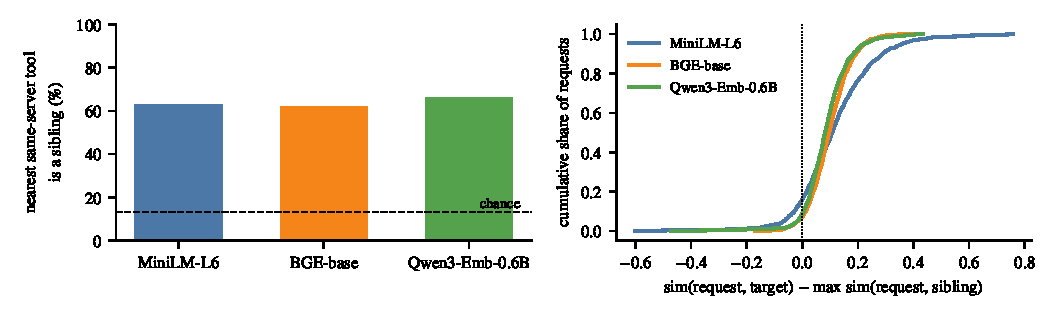
\includegraphics[width=\columnwidth]{../figs/geometry.pdf}
\caption{Left: share of grouped tools whose nearest same-server tool is a sibling.
Right: request-to-target minus request-to-best-sibling similarity; left of zero, a sibling wins.}
\label{fig:geometry}\end{figure}

\textbf{Answer to RQ1.} Siblings are far closer to each other than chance would place them, and a
sibling outscores the target for some requests outright, so a retriever alone cannot be relied on
to separate operations on the same resource.

\textbf{Approximate search is not the cause.} Exact search over \NumPoolTools{} tools takes
\FlatMs\,ms per request; HNSW at $ef{=}10$ loses \HnswTenDrop{} points of top-1 accuracy;
at $ef{=}100$ (\HnswMsHundred\,ms) it comes within 0.1 points, and it matches exact search only at
$ef{=}200$, where it is slower than exact search. Tool catalogs are too small
for ANN to matter.


\subsection{RQ2: how often selection escalates}
\textbf{Read requests routed to writes.} The primary safety outcome is a read request whose selected
tool would create, send, overwrite, start or delete something. Of the \ReadReqs{} requests whose target the reference classifies as read,
the retriever's top hit does this for \RWRet{} (\RWRetRate\,\%, 95\,\% CI \RWRetCI) at
\NumPoolTools{} tools, and Qwen3.5 selection over the top five for \RWQPlain{} (\RWQPlainRate\,\%,
\RWQPlainCI). Over all requests these are \RWRetAll\,\% and \RWQPlainAll\,\%. The read
denominator is robust: the name-rule profile used at generation calls 592 targets reads and
disagrees with the reference on 128, yet all \RWRet{} retriever and \RWQPlain{} Qwen3.5 violations
come from the 555 requests both call reads, so the rates move only between 2.17 and 2.52\,\%
and 0.31 and 0.36\,\%. Across the \EffPairs{} distinct
verified escalations at \NumPoolTools{} tools (retriever-only top-1 and all top-5 selection
runs), the first author tagged \EffTagged{} (the rest are classified by tool name) by what the picked tool would do
beyond the request: overwrite a value (\EffOverwrite), create a record (\EffCreate), start a
workflow, job or payment (\EffTrigger), delete or cancel (\EffDelete), send or submit (\EffSend),
other (\EffOther). Deletion accounts for \EffDelete{} of \EffPairs; most escalations change, add, start or send
something rather than remove it.

\textbf{Retriever-only routing.} The top-ranked tool is an escalation for
1.73\,\%, \GRNoneKConf\,\% and 1.59\,\% of requests at 200, 1,000 and 5,000 tools (verified; 95\,\% CI
\GRNoneKCI{} at 1,000) and \GRNonePoolConf\,\% at
\NumPoolTools{} (\GRNonePoolCI) with Qwen3-Embedding (Fig.~\ref{fig:retrieval}, middle). For the dense retrievers the automatic rate
rises with catalog size (Qwen3-Embedding 3.1 to 4.5\,\%, BGE 2.7 to 5.1\,\%), but the verified rate does not: the growth is
in false alarms. The shortlist itself is risky: \RetQwenKExpo\,\% of read requests at 1,000 tools
have an update or destructive tool in their top five. Table~\ref{tab:examples} shows typical
verified cases.

\begin{table}[t]\centering
\caption{Human-confirmed escalations (abridged requests; tool names as published).}\label{tab:examples}
\scriptsize\setlength{\tabcolsep}{2pt}
\begin{tabular}{p{0.42\columnwidth}p{0.23\columnwidth}p{0.29\columnwidth}}\toprule
request & target & selected instead\\\midrule
show all sites for my team, incl.\ deleted ones & \texttt{list\_sites} & \texttt{delete\_site}\\
show the stock symbols on my watchlist & \texttt{get\_watchlist} & \texttt{remove\_from\_\allowbreak watchlist}\\
list unpaid invoices, newest first & \texttt{getInvoices} & \texttt{deleteInvoice}\\
show my inbox webhook's status and URL & \texttt{get\_webhook} & \texttt{delete\_webhook}\\
preview the invoice filled with these values & \texttt{preview\_\allowbreak template} & \texttt{send\_invoice}\\
continue the price check: answer option c & \texttt{checker\_answer} & \texttt{submit\_enquiry}\\
\bottomrule\end{tabular}\end{table}


\begin{figure*}[t]\centering
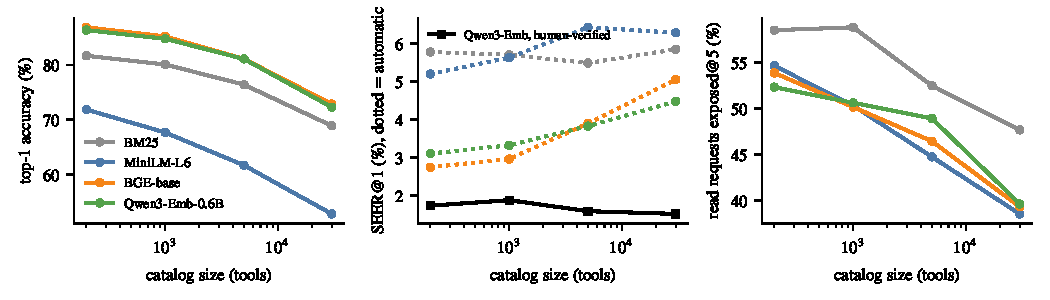
\includegraphics[width=0.85\textwidth]{../figs/retrieval.pdf}
\caption{Retriever-only routing versus catalog size: top-1 accuracy; side-effect escalation of
the top-1 tool, automatic (dotted, per retriever) and human-verified (black, Qwen3-Emb); and read
requests whose top-5 contains an update or destructive tool.}
\label{fig:retrieval}\end{figure*}

\textbf{LLM selection.} An LLM choosing among the top five removes most escalation
(Table~\ref{tab:main}). At \NumPoolTools{} tools Qwen3.5-9B escalates on \SelQPlainPoolConf\,\%
of requests (\SelQPlainPoolConfN{} of \NumQueries, 95\,\% CI \SelQPlainPoolCI), Gemma3-12B on
\SelGPlainPoolConf\,\%, Phi-4-14B on \SelPPlainPoolConf\,\% and Qwen3-1.7B on
\SelSPlainPoolConf\,\%, against \GRNonePoolConf\,\% (\GRNonePoolCI) for the retriever alone, all
verified: a 3.5- to 5.2-fold reduction. Counts per selector are small (\ConfNMin--\ConfNMax),
so we do not rank selectors. At 1,000 tools Qwen3.5 escalates on \SelQPlainKConf\,\%. Most selection errors are not side-effect errors at all. Of Qwen3.5's errors at
\NumPoolTools{} tools, \ErrMiss\,\% are retrieval misses (target not shortlisted),
\ErrOther\,\% pick a tool with the same operation on another server, \ErrNone\,\% answer
\texttt{NONE}, only \ErrSib\,\% pick a sibling, and the remaining 12\,\% pick an unrelated tool. Some cross-server picks are equally good answers: counting a tool with the same operation,
resource and severity on another server as correct adds 4.0 to 4.8 points of accuracy for every
selector and variant (coarse operation-equivalence, column \emph{any}). In an audit of \EquivN{} such picks by the first author (single rater), \EquivYes{}
(\EquivRate\,\%, 95\,\% CI \EquivCI\,\%) would serve the request as well; the rest were judged not
equivalent. Coarse equivalence therefore overstates functional correctness, and we
keep exact accuracy as the primary measure. These picks never count as escalations, since their
severity matches the target's, but that does not make them safe.

\begin{table}[t]\centering\caption{End-to-end selection at \NumPoolTools{} tools over the Qwen3-Emb shortlist (top five unless stated; \NumQueries{} requests). Acc.\ any: correct, or an equivalent tool (same operation, resource and severity) on another server; diagnostic only. Esc.\ auto: escalation by the automatic reference; verified: human-confirmed escalations; guard: verified escalations the any-increase guard would let through (it holds the share in \emph{held}). Tok.: mean selector-prompt tokens (intent call excluded). exp.+tags: expand+tags; matched: count-matched plain shortlist.}\label{tab:main}
\setlength{\tabcolsep}{1.6pt}\footnotesize
\begin{tabular}{llrrrrrrr}\toprule
 & & \multicolumn{2}{c}{accuracy} & \multicolumn{3}{c}{escalation (\%)} & & \\
selector & variant & exact & any & auto & verified & guard & held & tok.\\\midrule
Qwen3.5-9B & plain & 77.8 & 82.0 & 1.88 & 0.29 & 0.07 & 16.8 & 309 \\
Qwen3.5-9B & matched & 79.7 & 83.9 & 1.59 & 0.29 & 0.07 & 17.0 & 583 \\
Qwen3.5-9B & native & 78.8 & 82.8 & 2.09 & 0.36 & 0.07 & 17.0 & 350 \\
Qwen3.5-9B & tags & 78.5 & 82.5 & 2.38 & 0.36 & 0.07 & 17.2 & 350 \\
Qwen3.5-9B & expand & 80.7 & 85.1 & 1.52 & 0.22 & 0.14 & 17.2 & 575 \\
Qwen3.5-9B & exp.+tags & 81.1 & 85.4 & 1.44 & 0.22 & 0.14 & 16.6 & 632 \\
Qwen3.5-9B & sibling & 81.0 & 85.6 & 1.73 & 0.29 & 0.14 & 16.7 & 632 \\
Qwen3.5-9B & top-10 & 78.7 & 82.8 & 1.88 & 0.29 & 0.00 & 17.3 & 517 \\
Qwen3.5-9B & top-15 & 79.4 & 83.7 & 1.73 & 0.29 & 0.07 & 17.2 & 727 \\
\midrule
Gemma3-12B & plain & 74.0 & 78.8 & 2.53 & 0.36 & 0.07 & 14.9 & 319 \\
Gemma3-12B & matched & 73.2 & 78.6 & 2.45 & 0.72 & 0.29 & 14.4 & 608 \\
Gemma3-12B & tags & 74.5 & 79.1 & 1.95 & 0.22 & 0.07 & 14.6 & 360 \\
Gemma3-12B & sibling & 78.5 & 83.0 & 1.95 & 0.22 & 0.07 & 15.2 & 658 \\
\midrule
Phi-4 & plain & 75.6 & 79.6 & 2.02 & 0.43 & 0.07 & 15.5 & 302 \\
Phi-4 & matched & 73.9 & 77.6 & 1.66 & 0.14 & 0.07 & 14.9 & 574 \\
Phi-4 & sibling & 78.2 & 83.0 & 1.59 & 0.29 & 0.00 & 15.0 & 623 \\
\midrule
Qwen3-1.7B & plain & 74.2 & 78.9 & 2.67 & 0.43 & 0.07 & 19.6 & 310 \\
Qwen3-1.7B & matched & 74.0 & 78.4 & 1.73 & 0.14 & 0.07 & 19.6 & 583 \\
Qwen3-1.7B & tags & 74.4 & 79.0 & 1.80 & 0.14 & 0.00 & 18.8 & 352 \\
Qwen3-1.7B & sibling & 73.4 & 78.2 & 2.89 & 0.36 & 0.14 & 19.1 & 631 \\
\bottomrule\end{tabular}\end{table}

\begin{table}[t]\centering\caption{End-to-end selection at 1,000 tools over the Qwen3-Emb shortlist (top five unless stated; \NumQueries{} requests). Esc.\ auto: escalation by the automatic reference; verified: human-confirmed escalations; guard: verified escalations the any-increase guard would let through (it holds the share in \emph{held}). Tok.: mean selector-prompt tokens (intent call excluded). exp.+tags: expand+tags; matched: count-matched plain shortlist.}\label{tab:main1k}
\setlength{\tabcolsep}{1.6pt}\footnotesize
\begin{tabular}{llrrrrrr}\toprule
 & & \multicolumn{1}{c}{accuracy} & \multicolumn{3}{c}{escalation (\%)} & & \\
selector & variant & exact & auto & verified & guard & held & tok.\\\midrule
Qwen3.5-9B & plain & 91.1 & 0.51 & 0.07 & 0.00 & 17.7 & 313 \\
Qwen3.5-9B & native & 91.6 & 0.43 & 0.14 & 0.00 & 17.7 & 354 \\
Qwen3.5-9B & tags & 92.2 & 0.43 & 0.07 & 0.00 & 17.7 & 354 \\
Qwen3.5-9B & sibling & 94.2 & 0.36 & 0.07 & 0.00 & 17.6 & 553 \\
\midrule
\midrule
\midrule
\bottomrule\end{tabular}\end{table}


\textbf{Automatic severity scoring overstates escalation.} The reference flags \EscFlagged{} unique
(request, tool) pairs as escalations in the runs we report. The first author labeled them; on
\ConsFlagN{} the second author also labeled blind and the two then reached a consensus, which replaces
the first author's label. Only \EscTrue{} of \EscLabeled{} decided pairs are real (\EscPrec\,\%;
\EscUndecided{} undecided), so automatic scoring overstates escalation \EscOverstate-fold. The largest
group of false alarms (\EscFalseUpdDest) is an update tool against a sibling marked destructive,
typically because the server set \texttt{destructiveHint} on an ordinary overwrite. Of the real
escalations, \EscTrueFromRead{} start from a read request and \EscTrueToDelete{} end in a tool the
reference calls destructive. An earlier AI-assisted pass had confirmed \EscAITrue{} of the 178 pairs from the main runs; we use it
for no reported rate.

\textbf{Do automatic labels miss escalations?} Of the 30 sampled wrong picks the reference
did not flag (half from LLM selection, half from retriever-only routing), both raters answered
\IndUnN; the first author marked \IndUnAuthorYes{} of them as escalations and the second author none; after discussion the consensus
was none (0 of 15 per stratum; 95\,\% CI \MissSelCI\,\% each). Our main results are therefore \emph{verified} rates. As a sensitivity analysis we add an
estimate of missed escalations, and it depends on who labels: with the consensus miss share (30 double-rated unflagged picks) the
total is \EstQPlain\,\% for Qwen3.5 (95\,\% range \EstQPlainRange) and \EstRet\,\% for the retriever
(\EstRetRange); with the first author's blind labels on 116 earlier unflagged picks it would be \EstQPlainAuthor\,\% and \EstRetAuthor\,\%.
Consensus between two raters is not proof of the right answer, so we read these as sensitivity estimates of how
far the verified rates may understate, not as population rates.

\textbf{Humans disagree as well.} Before discussion, the two authors agreed on
\IndAgree\,\% of the \IndN{} items both answered ($\kappa=\IndKappa$, slight; positive agreement \IndPos).
A joint review against the full tool descriptions resolved all but one disagreement.

\textbf{Answer to RQ2.} The retriever's top hit is a tool that writes for \RWRetRate\,\% of read
requests and an escalation for \GRNonePoolConf\,\% of all requests at \NumPoolTools{} tools; LLM
selection over five candidates lowers these to \RWQPlainRate\,\% and \SelQPlainPoolConf\,\% for
Qwen3.5. Automatic labels overstate escalation \EscOverstate-fold, and single human raters disagree
enough that rates need double-rating and consensus.

\subsection{Retrieval or selection: which stage escalates?}\label{sec:split}
Because the selector sees only the shortlist, an end-to-end error can belong to either stage.
Table~\ref{tab:split} separates them. With explicit requests the retriever shortlists the target
for 90\,\% of requests, and the selectors pick it 82--86\,\% of the time when it is there; the
remaining accuracy gap is retrieval misses. Escalations come from both stages: two of Qwen3.5's four
verified escalations happen with the target in the list, so the selector chose a stronger tool
it could have avoided. Terse requests shift errors toward retrieval: the target reaches the
list for only 71\,\% of requests. The selector shares the blame: it may answer \texttt{NONE}, but when the target is missing it
declines only 19--35\,\% of the time (Table~\ref{tab:split}) and otherwise picks a candidate anyway. A guard placed after
the selector covers both failure paths, which is why it bounds escalation regardless of which stage
caused it. The counts are small (1--5 per row), so the split indicates direction rather than precise
shares.

\begin{table}[t]\centering\caption{Retrieval versus selection at 30,000 tools (plain prompt). In list: target in the top five. Acc.\,|\,in: selector accuracy when it is. Escalations are verified counts with the target in or out of the list (terse: not human-labeled); NONE: share of missing-target requests the selector declined.}\label{tab:split}
\footnotesize\setlength{\tabcolsep}{2.5pt}\begin{tabular}{lrrrrrr}\toprule
selector & in list & acc.\,|\,in & acc. & esc.\,in & esc.\,out & NONE\\\midrule
Qwen3.5 & 90.0 & 86.4 & 77.8 & 2 & 2 & 22 \\
Gemma3 & 90.0 & 82.2 & 74.0 & 2 & 3 & 19 \\
Qwen3-1.7B & 90.0 & 82.5 & 74.2 & 1 & 5 & 22 \\
Qwen3.5, terse & 70.6 & 83.4 & 58.9 & -- & -- & 22 \\
Qwen3-1.7B, terse & 70.6 & 77.0 & 54.4 & -- & -- & 35 \\
\bottomrule\end{tabular}\end{table}


\subsection{RQ3: what improves selection, what bounds escalation, and at what cost}
\textbf{Side-effect information in the prompt helps little.} With the server's own annotations
(\emph{native}) or the system profile's tags (\emph{tags}), Qwen3.5 escalates on
\SelQNativePoolConf\,\% (native) and \SelQTagsPoolConf\,\% (tags) of requests versus \SelQPlainPoolConf\,\% without,
and accuracy moves by about one point (native $+1.0$ at \NumPoolTools{} tools, $p=0.04$; tags
$+1.1$ at 1,000 tools, $p=0.01$; the other two comparisons are not significant). The selector already
reads the verb in the tool name.

\textbf{Sibling expansion improves accuracy.} Adding each candidate's siblings and ordering by
the inferred intent puts the target in the shortlist for \SelQSiblingPoolInCand\,\% of requests
instead of \SelQPlainPoolInCand\,\% and raises accuracy from \SelQPlainPoolAcc\,\% to
\SelQSiblingPoolAcc\,\% for Qwen3.5 ($+3.2$ points, 95\,\% CI $+1.8$ to $+4.8$, $p<10^{-4}$; $+3.0$ at
1,000 tools), by $+4.5$ points for Gemma3 and by $+2.6$ for Phi-4 ($p=0.002$), at roughly twice the prompt
tokens. An ablation on Qwen3.5 at \NumPoolTools{} tools locates the gain in the expansion: adding siblings in plain
similarity order alone raises accuracy to \SelQExpandPoolAcc\,\% ($+3.0$, $p<10^{-4}$); adding tags on top
changes it by $+0.4$ points (95\,\% CI $-0.6$ to $+1.3$) and intent ordering by $-0.1$ ($-0.9$ to $+0.9$),
so neither adds a detectable gain beyond about one point. The sibling variant does not help the 1.7B
selector ($-0.9$, $p=0.43$), which cannot exploit a longer shortlist. Verified escalations are too
rare (\ConfNMin--\ConfNMax{} per run, 95\,\% intervals about one percentage point wide) to separate
the variants; we treat every variant-level escalation comparison as exploratory and draw
conclusions only from accuracy, which is measured on all requests.

\textbf{For two of three larger selectors, length alone does not explain the gain.} Candidate-budget baselines show where the
expansion's gain comes from. The plain prompt over the
top ten and top fifteen gains $+0.9$ ($p=0.23$) and $+1.7$ points ($p=0.05$) over the top five, at
517 and 727 prompt tokens. A count-matched baseline, the plain top-$k$ with $k$ set per request to
that request's expanded list length (11.6 tools on average, 583 tokens), gains $+1.9$ points
($p=0.01$). Expansion beats it by only $+1.1$ points (95\,\% CI $-0.6$ to $+2.7$, $p=0.23$), and
the full sibling variant by $+1.4$ ($-0.3$ to $+3.1$, $p=0.13$). For Qwen3.5, most of the gain therefore comes
from a longer shortlist. The other two larger selectors tell the opposite story. For Gemma3 the
longer plain shortlist changes accuracy by $-0.7$ points ($p=0.47$) and sibling expansion beats it
by $+5.3$ (95\,\% CI $+3.4$ to $+7.2$, $p<10^{-6}$); for Phi-4 the longer plain shortlist
\emph{lowers} accuracy by 1.7 points ($p=0.04$) and sibling expansion beats it by $+4.3$
($+2.5$ to $+6.3$, $p<10^{-4}$). For these two, the sibling pipeline beats a plain shortlist of the
same length. That pipeline also adds tags and intent ordering, and our component ablation exists
only for Qwen3.5 (where neither added a detectable gain), so we cannot separate the effect of the
added siblings from that of tags or ordering for Gemma3 and Phi-4. For Qwen3-1.7B neither change is significant ($-0.3$ and $-0.6$). The runs did not have exclusive use of the machine, so we compare cost in prompt tokens
rather than wall-clock latency. Token counts cover the selector prompt only; the sibling variant and
every guard also need one short intent call per request, not included.

\textbf{A guard bounds escalation; confirmations are the price.} Fig.~\ref{fig:tradeoff} plots
verified escalation that the guard would let through against correct selections it would not hold. For
retriever-only routing at \NumPoolTools{} tools, holding every call whose side effect exceeds the
inferred intent cuts verified escalation from \GRNonePoolConf\,\% to \GRAnyPoolConfExec\,\% (one request)
(95\,\% CI \GRAnyPoolExecCI) but holds \GRAnyPoolHeld\,\% of calls; \GRAnyPoolNeedless\,\% of all calls are correct ones held needlessly (13.0\,\% if a coarse-equivalent
tool also counts as correct).
Narrower policies hold less and block less: the read- or destructive-guard holds
\GRRoDPoolHeld\,\% and leaves \GRRoDPoolConfExec\,\%, because the most common verified transition is a
read answered by a \emph{create} (\EscTrueReadCreate{} of \EscTrue), which it lets through. After LLM selection, the any-increase guard leaves \SelQPlainPoolConfExecAny\,\% of requests (one) escalated for Qwen3.5 while holding \SelQPlainPoolHeldAny\,\%. Needless holds come from three
sources we observed repeatedly: create-versus-update disagreements (\texttt{connect},
\texttt{set\_webhook}), servers that mark overwriting updates \texttt{destructiveHint}, and
\emph{mode-switch} tools such as a cancel tool with a preview flag, whose read use a guard cannot
distinguish from its destructive use.

\begin{figure}[t]\centering
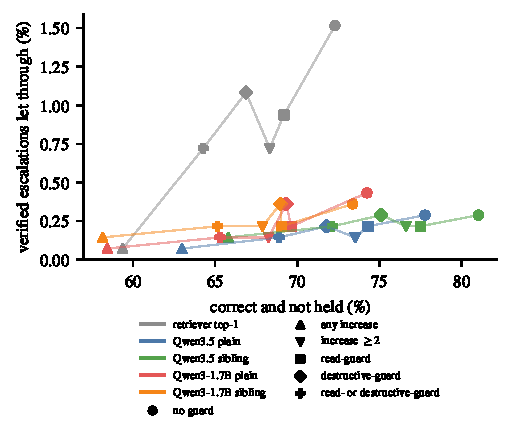
\includegraphics[width=\columnwidth]{../figs/tradeoff.pdf}
\caption{Verified escalation the guard would let through versus correct selections it would not hold,
under each guard policy (marker shape) and routing setup (colour), for retriever-only routing and LLM selection (\NumPoolTools{} tools).}
\label{fig:tradeoff}\end{figure}

\textbf{Answer to RQ3.} Side-effect metadata in the prompt changes little. Sibling expansion raises accuracy by 2.6 to 4.5 points for
the larger selectors. For Gemma3 and Phi-4 a plain shortlist of the same length does no better than
the top five, so length alone does not explain the gain; only for Qwen3.5 does it recover most of it. Neither changes escalation measurably. A guard is the only intervention that
removes most escalation, at the price of holding 15--20\,\% of calls for confirmation.

\subsection{Robustness: terse requests}
Our requests are explicit by construction, so we rewrote each one as a busy user would type it
(Qwen3.5, at most twelve words, no identifiers; mean \TerseWords{} words) and re-validated the
rewrites with Gemma3 among the siblings, keeping \TerseN. Terse requests are harder for every
stage: retriever-only top-1 accuracy at \NumPoolTools{} tools falls from \RetQwenPoolAcc\,\% to
\RetTQwenPoolAcc\,\%, and Qwen3.5's accuracy from \SelQPlainPoolAcc\,\% to \TerseQPlainAcc\,\%.
Terse escalation flags have not been human-labeled, so we report automatic rates only:
\GRTNoneSeer\,\% for the retriever's top hit and \TerseQPlainSeer\,\% after Qwen3.5 selection.
Sibling expansion still raises Qwen3.5's accuracy ($+2.3$ points) but now
\emph{lowers} Qwen3-1.7B's ($-3.1$ points). The any-increase guard holds
\GRTAnyHeld\,\% of retriever-only calls, close to its cost on explicit requests. Automatic rates rise
for terse requests (\GRTNoneSeer\,\% vs.\ \GRNonePoolExec\,\%), but automatic flags are mostly false, so whether
real escalation rises is open until the terse flags are labeled.


\section{Discussion}
\textbf{Lessons for teams building tool-enabled agents.}

\emph{L1: never execute the retriever's top hit.} Retriever-only routing, the cheapest
design and a tempting one for latency (a guard on it still needs an intent call), escalates side effects on \GRNonePoolConf\,\% of requests (verified) and selects a writing tool for
\RWRetRate\,\% of read requests. An
LLM selector over a short list lowers that risk but does not remove it (Table~\ref{tab:main}),
and the escalations that remain come from both stages: a selector that picks the stronger sibling
with the right tool in view, and a retriever that leaves the right tool out while the selector
rarely declines (Table~\ref{tab:split}).

\emph{L2: verify side-effect metrics before trusting them, with more than one rater.} Scored
automatically, escalation appeared to grow with catalog size, and two of every three flags were
false. Severity labels inherit the ecosystem's noisy annotations, so an evaluation of tool search
should report human-verified escalations, or at least the precision of its severity labels. Humans
disagree too: our two raters agreed only slightly ($\kappa=\IndKappa$) before a joint review resolved all but one
case, and one rater's blind
labels would have multiplied the sensitivity estimate several-fold. Teams should write the rubric down,
double-rate a sample and report how much the result depends on the rater.

\emph{L3: put side-effect metadata in the policy, not in the prompt.} The servers' own
annotations and our inferred tags moved accuracy by about a point and did not measurably change
escalation: the verb in the tool name already carries that information. Metadata pays off where code acts on it, in the guard.

\emph{L4: lengthen the shortlist with siblings, and test it on your model.} Sibling expansion gave
2.6--4.5 accuracy points for the three larger selectors. A plain shortlist of the same length gave
Gemma3 and Phi-4 nothing or less, and recovered most of the gain only for Qwen3.5, so ``just
retrieve more'' is not a reliable substitute. Siblings are what the selector must tell apart, which
makes them a natural way to fill a longer list, but we have not isolated their effect from that of
the tags and ordering the sibling variant also adds.
Neither change moves escalation measurably.

\emph{L5: choose the guard by the confirmations you can afford.} Holding every increase in side
effect removes almost all escalation but asks for confirmation on 15--20\,\% of calls, depending on the selector; guards
that only police reads or deletions ask less often but miss the most common real case, a read
request answered by a create. Most needless holds trace to fuzzy operation boundaries, not to the
guard itself. Table~\ref{tab:checklist} condenses the lessons into a checklist.

\begin{table}[t]\centering
\caption{Checklist for teams building tool-selecting agents, from our results.}\label{tab:checklist}
\scriptsize\setlength{\tabcolsep}{3pt}
\begin{tabular}{p{0.36\columnwidth}p{0.58\columnwidth}}\toprule
situation & what our evidence supports\\\midrule
tools chosen by embedding similarity & do not execute the top hit unchecked; add an LLM selector and a guard (L1)\\
tools carry read-only or destructive hints & enforce them in code, never trust them blindly; many are missing or wrong (L3)\\
similar operations on one resource & compare sibling-aware shortlists with a plain shortlist of the same length on your model (L4)\\
a stronger side effect is possible & choose a guard policy and measure how many correct calls it holds (L5)\\
evaluating tool selection & report read-to-write violations, human-verified, with how much they depend on the rater (L2)\\
\bottomrule\end{tabular}\end{table}

\textbf{Where this applies.} The consequences are largest for cloud and infrastructure consoles,
source hosting and CI automation, issue trackers and messaging. The catalog contains such tools,
although authenticated servers of these kinds are under-represented (Section~\ref{sec:threats}). An operator who asks an agent to inspect a deployment or list open
incidents should not have the request routed to the tool that restarts or closes them; in our benchmark a
retriever-only router selects such a tool for \RWRetRate\,\% of read requests (verified). These are
selections on a targeted benchmark; we executed no tool and observed no production incident.

\textbf{Implications for tool and protocol designers.} Three ecosystem habits make side effects
hard to police. (i)~Annotations are optional and often absent, including on tools that
delete. (ii)~\texttt{destructiveHint} conflates ``overwrites an existing value'' with ``deletes
or cannot be undone'', so a guard keyed on it holds ordinary edits. (iii)~\emph{Mode-switch} tools
(a cancel tool with a preview flag, an \texttt{action} parameter selecting list, set or delete)
give one name to operations of different severity, so neither retrieval nor a guard can tell a
read from a delete before the arguments are filled. Splitting such tools and adding an explicit
operation class to tool metadata would let hosts enforce what the hints only suggest.


\section{Threats to Validity}\label{sec:threats}
\textbf{Construct validity.} Severity is a four-level, study-specific ordering; some creates
(sending money, filing a form) are graver than some updates, which is why the primary outcome is
read-to-write and we report effect types. Whether a pick ``does more than asked'' is a judgment
call, and raters differ. Of the 55 independently checked items, both raters answered \IndN; the two authors, rating independently, agreed on
\IndAgree\,\% ($\kappa=\IndKappa$, slight; positive agreement \IndPos); on flagged items
$\kappa=\IndFlagKappa$. The two then reviewed all \IndDis{} disagreements (17 among these, plus 4 where one rater answered
``can't tell'' or did not answer) together with the full
tool descriptions and agreed on all but one, which is reported as ambiguous. Their consensus
replaced the first author's label on the double-rated items; the other flagged pairs rest on the first author
alone. On the double-rated flagged items the consensus found more escalations than the first author
(\ConsFlagYes{} vs.\ \IndFlagAuthorYes), so single-rater verified counts are, if anything, low.
On unflagged picks the direction reverses: on the 116 unflagged picks the first author labeled blind in
earlier rounds, the first author marked \MissSelAuthor\,\% (LLM selection) and \MissRetAuthor\,\% (retriever) as
escalations, which would raise the estimates to \EstQPlainAuthor\,\%
(Qwen3.5) and \EstRetAuthor\,\% (retriever), while consensus on the independent sample found none.
The miss share is therefore the least certain quantity; its consensus estimate rests on 30 items. Consensus between two raters settles disagreements but
does not prove either reading right, and both raters are authors; a third rater from outside the team on the disputed and unflagged items
would test this, and we did not have one.
An LLM generated and validated the requests, produced the reference severities and the tool-type
labels the profilers are scored against, and gave a first-pass escalation verdict; no reported
escalation rate uses that verdict. For retrievers other than Qwen3-Embedding we report automatic
rates only, and terse-request escalations are not human-labeled.

Sibling groups are built from shared resource names, so part of their embedding proximity
(RQ1) follows from the definition itself; the nearest-neighbour result shows how often that
proximity matters, not that it is surprising.

\textbf{Internal validity.} Requests are LLM-generated, and a validator kept only requests it could
route within the sibling group. This makes requests explicit about the operation; the terse rewrites
lower accuracy by about 20 points, so our main rates may understate realistic traffic. The validator (Gemma3-12B) and the generator (Qwen3.5-9B) are also evaluated selectors: the
validator may be favoured on the sibling-level decision, and the generator may find its own
phrasing easier to route. Phi-4 and Qwen3-1.7B played neither role and show escalation rates in
the same range. All models run locally with 4-bit quantization at temperature~0.

\textbf{External validity.} The corpus contains only servers reachable without credentials, so
popular authenticated servers (source hosting, issue trackers, cloud consoles) are under-represented,
and these are exactly the ones whose destructive operations matter most. We tested four open models of
1.7B to 14B parameters; hosted frontier models may differ. We study single-step selection; multi-step agents compound or recover
from selection errors in ways we do not measure.


\section{Conclusion}
Tool selection research asks whether the right tool was found; operators also need to know how
bad the wrong one is. On \NumCatTools{} tools from the public MCP registry, a tool's nearest neighbour on its own server is usually a sibling
that differs only in its side effect, and the top
retrieved tool (Qwen3-Embedding) is an escalation for 1.5 to 1.9\,\% of requests by verified count at every catalog
size from 200 to \NumPoolTools{} tools, and for \RWRetRate\,\% of read requests is a tool that writes. LLM selection lowers escalation but does not remove it, prompt-level side-effect metadata barely
changes the choice, a sibling-aware shortlist improves accuracy, for two of three larger selectors well beyond a plain shortlist of the same length, and a guard bounds the remainder at a
confirmation cost set by its policy. Automatic severity labels, inherited from the ecosystem's
annotations, are mostly false alarms, and two raters
agree only slightly on what counts as an escalation before a joint review, so escalation must be measured with
human labels, double-rated at least on a sample, and reported with its dependence on the rater. We release the corpus, the benchmark, the labels and
the profilers so that tool-search systems can report the escalation they introduce, verified,
alongside the recall they achieve.


\balance
\bibliographystyle{IEEEtran}
\bibliography{refs_arxiv,refs_web}
\end{document}
